\documentclass{article}
\usepackage[T1]{fontenc}
\usepackage{lmodern}
\usepackage{graphicx}
\usepackage{amsmath,amssymb}
\usepackage[a4paper,margin=2cm]{geometry}
\usepackage[absolute,overlay]{textpos}
\setlength{\TPHorizModule}{1mm}
\setlength{\TPVertModule}{1mm}
\usepackage[indonesian]{babel}
\usepackage{hyperref}
\setlength{\emergencystretch}{2em}
% unit: Halaman 55

\begin{document}

% === Halaman 55 (llm) ===

Enkripsi

\vspace{10mm}

\textbf{Crypt-Online}

Main $\Rightarrow$ Conversions $\Rightarrow$ RC4

\textbf{Encryptions}
\begin{itemize}
    \item Without a key
    \item Symmetric
    \begin{itemize}
        \item AES (Rijndael)
        \item DES
        \item RC4
    \end{itemize}
    \item Asymmetric
    \item Mathematical
    \item Utilities
\end{itemize}

% deskripsi: Screenshot antarmuka web encryptor RC4 yang menunjukkan input teks 'Terbanglah sampai ke angkasa setinggi bintang di langit', kunci 'Selamat sore gaess', dan hasil cipher text.
% bbox normalisasi: [0.2800, 0.3600, 0.7300, 0.9400]
\begin{textblock*}{94.50mm}(58.80mm,106.92mm)
\noindent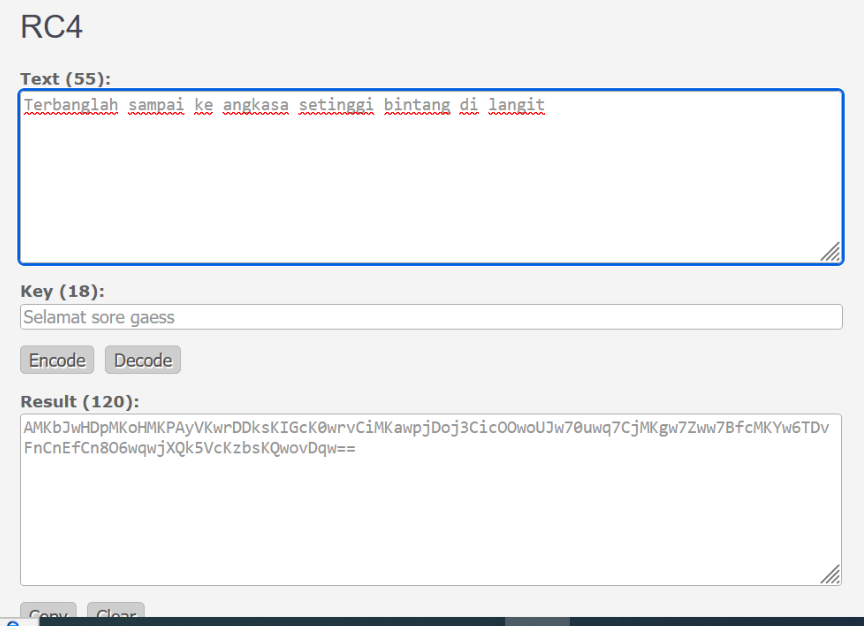
\includegraphics[width=94.50mm,height=172.26mm]{../../images/llm/page_055_img_01.png}%
\end{textblock*}

\end{document}
